\chapter{Compressive Sensing Theory}
%Real world signals are usually continuous time, to process these signals in the digital devices , it is essential to convert them into digital domain.This conversion is done with the help of sampling in which signal is reduced by measuring at certain intervals in time. In order to reconstruct the signal from its samples efficiently, sampling theorem was presented by Shannon in 1949. According to $sampling theorm$, in order to perfectly recover the signal, the sampling rate must be twice the maximum frequency present in the signal. Although, shannon's theorem provide a vital bridge between continuous time and discrete time signal and has been proved extremely fruitful but it consider idealistic scenarios while reconstructing\cite{sampling_theorm}.For example, practically signal are never exactly band-limited and their is no ideal low pass filter.In \cite{under_samping} D. L. {Donoho} and J. {Tanner} states that $sampling therom$ is wrong and presented a systematic framework for under-sampling phenomena. Undersampling theorems affirms that a signal/image can be reconstructed perfectly by considerably fewer samples than the conventional sampling theorem, condition provided that the signal must be sparse in nature.

%\textit{Compressed sensing} or  \textit{Compressive sensing} (CS), is a path breaking signal processing based technique, which provides theoretical guarantees for efficiently acquiring an undersampled signal and reconstructing it, by finding solutions to underdetermined linear system.
%This framework is based on compressing the signal while sensing it, in opposite to conventional  compression techniques like JPEG, where the signal/image is first acquired at a high sample rate and then compression is applied. It is based on the fact that as in sparse signals most of the entries are zero, therefore, it is inefficient to invest lots of power to observe them. The objective of CS is to estimate the original signal from linear incoherent compressed measurements.

Data acquisition is one of the most significant steps in any data processing pipeline.  Real-world signals are continuous-time, while processing on them is done on digital platforms. To process continuous time on digital platforms, the signals are quantized and sampled. The process of sampling should be reversible, this implies that the signal should be reconstructable after being sampled. To enable accurate reconstruction from samples, according to Shannon theorem the signal should be sampled at least twice the maximum frequency of the signal. However, the maximum frequency in real world signal is very high, this demands higher sampling rate to meeting nyquist criterion. Once sampled, the signal is processed resulting in data, this data must be stored digitally. Therefore, with higher rate of sampling the data must be compressed to enable efficient storage. The major disadvantage in data acquisition and storage compression is discarding lot of data which was sensed. That means that data was oversampled while sensing it at first place, after that point large amount of sensed data is discarded to enabled efficient storage.  Another intuitive way to achieve more efficiency would be to sense the data in a compressive way and then try to recover the signal from this compressed data, such technique is known as \textit{Compressed sensing} or  \textit{Compressive sensing} (CS). 
\section{Review of Sparsity and Compressibility}
Compressive sensing involves sensing signal in compressed form also known as observation y and estimating the signal $x$ using it. To ensure correct estimation of signal from the observations the data is compressed using special noise like waveforms extracted from matrix $A$ also known as sensing matrix or measurment matrix. The idea is to acquire $y$ in the way that it is represented using the basis of  $A$ and while recovering x search the appropriate combination of columns of  $A$ projected on $x$.  
\begin{equation}
    y=A^T x
\end{equation}
%The compressive sensing system is, however, the underdetermined system since the unknown variables are larger than the number of equations. 
Consider the size of observation $y$ is $M \times 1$ and size of to be estimated signal $x$ be $N \times 1$ and  $A$ is the matrix of size $M \times N$. 
Here, an important point to notice is that as $M\ll N$ therefore it is an undetermined system\footnote{In mathematics, linear equation system states that a system is underdetermined if the number of equations are less than number of unknowns} and exact solution to such system do not exist or the system will have infinite solutions. One way out of solving such an ill-posed system is by considering the compressed sensing paradigm as explained in \cite{Candes08}.Which explain that in such  situation signal can be recovered with no or very less loss if it is sparse in some domain.
%In this case $M \ll N$ constituting underdetermined system. To ensure recovery  of such an underdermined linear the $\frac{N}{M}\ge 1$  and also that the vector $x$ should be sparse, that means it should contain much more zeros then non zero entries.
%\begin{enumerate}
  %\item The vector $x$ should be sparse, that means it should contain much more zeros then non zero entries.
 % \item Measurements are not time-space measurements as in most data acquisition systems rather are done using noise-like waveforms.
%\end{enumerate}

%This means that either $x$ should be sparse directly in time domain or could be represented as a sparse signal in some domain. For example, images are not sparse in direct sense, however, the wavelet transform can represent images as the sparse signal. 

%\begin{equation}
  %  \bar{X}=A \alpha 
  %  \label{cs_eq}
%\end{equation}

%In the above equation $\bar{X}$ is the image, $\psi$  is measurement matrix and $\alpha$ are wavelet coefficients. If the matrix is not a sparse special type of procedure called \textit{sparsity enforcement} is used to ensure that $\bar{X}$ is sparse. If $\bar{X}$ is not sparse it is not possible to recover the signal from y. Finding the right linear combination of columns of  $\phi$ projected on $\bar{X}$ is an optimization problem which deploys different algorithms to find the exact solution of the underdetermined system.  


\section{Measurement Matrix}
For efficient and precise sparse signal reconstruction, the design of measurement matrix is very critical.It is usually a combination of random matrix  $\Phi$(i.e., i.i.d Gaussian or Bernoulli) and  transform matrix $\Psi$(i.e., Fourier transform, discrete cosine transform, wavelet transform).So the CS matrix or sensing matrix can be written as;
$A=\Phi \Psi$
In the field of signal processing, transformations provide powerful tools for handling signals with distinct properties.
The choice of these matrices depends on the application under consideration, for example, in wireless communication usually Fourier transform is considered while in image processing and audio signal processing wavelet transform are applied. Usually, such sparse transformations are redundant and are also called redundant dictionaries. It is called over-complete dictionary if number of columns are greater than number of rows. This over-complete dictionary provides more redundant bases for more accurate and guarantee signal recovery, condition provided that it follows Restricted Isometric Property(RIP) and mutual coherence as explained in next subsection.

\section{Conditions for Perfect Recovery}

\subsection{Restricted Isometric Property(RIP)}

To guarantee sparse signal recovery it is essential that the  sensing matrix must obeys  Restricted Isometric Property(RIP) which can be expressed as follows as given in \cite{candes,Candes08},
\begin{equation}
    (1-\delta_S{_{max}}) \|x\|_2^2 \le \| A x \|_2^2 \le (1+\delta_S{_{max}})\|x\|_2^2
\end{equation}
In the above equation $\delta_S{_{max}} $ is the constrained parameter  $\delta_S{_{max}} \in \{0,1\}$ . The CS matrix must satisfy RIP for successful signal recovery.
One possible solution to satisfy the RIP condition is to select CS matrix as a random matrix. It is proved in \cite{sensing_mat} that if CS matrix is i.i.d Gaussian, Bernoulli or partial random Fourier matrix, it will hold RIP.
Therefore, the CS-based signal recovery will be reliable if we design sensing matrix from a random matrix or a combination of random matrix and a particular transform\cite{sparse_channel, Candes08}.
 
 \subsection{Mutual Coherence}
 Other than RIP another important condition for accurate sparse signal recovery is that random basis $\Phi$ and transform basis $\Psi$ must be incoherent to each other. This relationship of mutual incoherence can be defined as;
 \begin{equation}
     \mu(\Psi, \Phi)= \sqrt{n}\textrm{ } \underset{{1\le i,j \le n} }{max}|\langle \Psi_i, \Phi_j \rangle|
 \end{equation}
 This relationship defines the maximum correlation between the elements of these two matrices and it range can be given as $ \mu(\Psi, \Phi) \in {1,\sqrt{n}}$ \cite{Candes08}
\section{ Reconstruction Algorithms}
After discussing the sensing matrix or measurement matrix design and sufficient conditions for signal recovery with a guarantee. In this section, we will explain the reconstruction algorithms which finds the sparse solution for an underdetermined system with the help of $l_p$ norm ${p=0,1,2}$ minimization
\begin{equation}
    \|(x_i)_{i \in N}\|_p= \sqrt[P]{\sum_{i\in N} |x_i|^p}
\end{equation}
\begin{itemize}
    \item \textbf{$l_0$ norm minimization}
    If we have the prior information that our signal is sparse, then $l_o$ norm is natural choice to find the  sparsest solution, by counting the non-zero entries in the sparse vector, under the error bound less than $\epsilon$. This can be written as;
    \begin{equation}
        min\|x\|_o \textrm{subject to} \|Ax -y\|_2 \le \epsilon
    \end{equation}
    Although $l_o$ norm provides the exact solution but it is a NP hard(non-deterministic polynomial-time) problem. Therefore, it is computationally very expensive due to exhaustive search, a better option is to relax it to $l_1$ norm.
     \item \textbf{$l_1$ norm minimization}
    Due to computational infeasibility of $l_0$ norm, the research focus is more toward relaxing $l_o$ and finding solution using $l_1$ norm minimization.
    \begin{equation}
        min\|x\|_1 \textrm{ subject to } \|Ax -y\|_2 \le \epsilon
        \label{l1-norn}
    \end{equation}
    \begin{figure}
    \label{norm-fig}
     \centering
     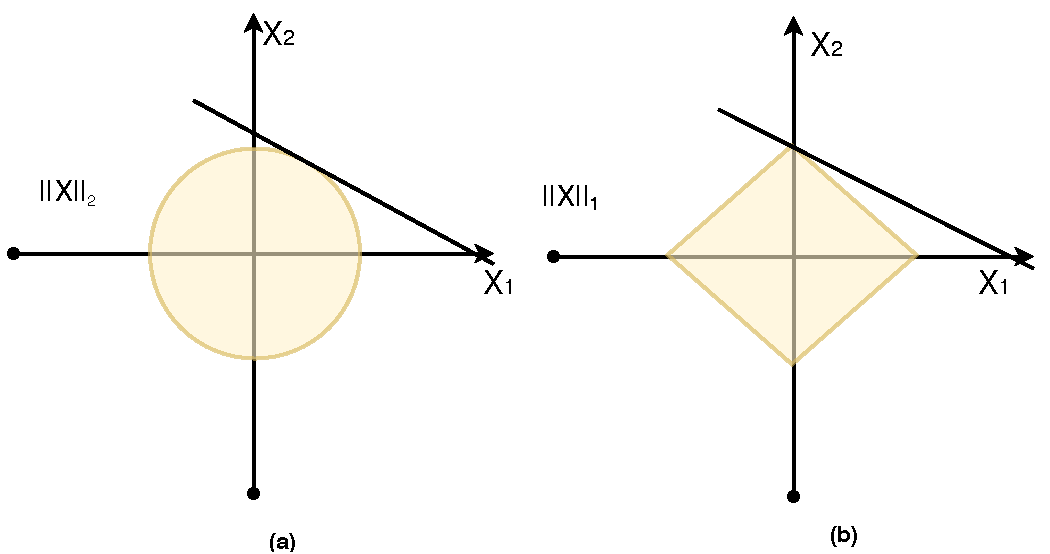
\includegraphics{figures/norm.pdf}
     { a) $L_2$ norm minimization}\hfil \hfil{ b) $L_1$ norm minimization}
 \end{figure}
    In the above figure \ref{norm-fig} graphical representation of $l_1$ norm minimization is shown. The objective of $l_1$ minimization is to find a sparse vector x in terms of minimum  of $\|x\|_1$ .The $l_1$ minimization is a convex program and can be solved using advanced optimization techniques like basic pusuit(BP),  least absolute shrinkage and selection operator(LASSO).
    \item \textbf{$l_2$ norm minimization}
    Other than, $l_1$ norm minimization in the literature $l_2 $ minimization is also used to find sparse approximation.
    In the figure \ref{norm-fig} the graphical view of $l_2$ minimization is shown. The $l_2$ minimization attempts to find out the sparsest solution  by minimizing  $\| x\|_2$  which can be achieved in general by the least square method.
    \begin{equation}
        min\|x\|_2 \textrm{  subject to } \|Ax -y\|_2 \le \epsilon
    \end{equation}
    In general, it is difficult to get the exact sparse vector by $l_2$ norm minimization even in the absence of noise. However, the  algorithms based on $l_2$ minimization are very popular because of their computationally less complexity and are called greedy algorithms(i.e.,orthogonal matching pursuit(OMP)).
\end{itemize}
Both algorithms based on $l_1$ and $l_2$ norm minimization are popular in the literature and have their own characteristics.  Hence, the choice of algorithm is dependent on the application under consideration. For the applications which require high level of accuracy as in medical applications, $l_1$ norm based algorithms could be a better choice but if the focus is more towards less computational complexity then greedy algorithms could be the best choice. Besides this, there are other popular algorithms which are based on thresholding for example iterative hard thresholding(IHT) and hard thresholding pursuit. In the following, we will discuss the algorithms based on convex optimization(BP), greedy algorithm(OMP) and also thresholding based algorithm(IHT and HTP).
\subsection{Convex Optimization based algorithm: Basic Puruit(BP)}
In this subsection we will discuss the convex optimization based very popular algorithm, basic pursuit(BP). This algorithm looks for global minima therefore, among several potential solutions to $y=Ax$,  it selects the one whose coefficients have a minimum  $l_1$ norm\cite{Donoho06}.
The simple form of basic pursuit using $l_1$ norm will do not work in  the presence of noise, therefore to suppress noise in the measurement we have to relax the inequality given in equation \ref{l1-norn} and the modified formulation will be called basic pursuit denoising(BPDN) as given below;
\begin{equation}
     min\|x\|_2 \textrm{  subject to } \frac{1}{2}\|Ax -y\|_2 \le \epsilon
\end{equation}

Different types of solvers have been used in the literature to acquire solution of such convex optimization based problem for example, BP-simplex, interior-point algorithm also known as BP-interior,fixed point continuation (FPC), gradient projection for sparse representation (GPSR).

\subsection{Greedy algorithms (Orthogonal Matching Pursuit (OMP))}
Orthogonal Matching Pursuit (OMP) is most popular greedy algorithm.
OMP projects the signal onto the subspace by the selecting atoms, limiting the same selection of atoms more than once.
In the first step a correlation is computed with all columns of $A$ and searched for highest correlation.  
 with $c_0=0$  $Res_o=y$
\begin{equation} \label{firstmax}
C_{t+1}= C_t \cup Arg max |A^T Res_t |
\end{equation}
where $C_t$ subset index for prominent indices, in each step $x_{t+1}$, $C_{t+1}$ is updated
Determine the orthogonal projection of $A^o$ onto
the span of the atoms indexed in $C_{t+1}$   ,
$A^o=(A_c)(A_c)^{\dagger}$
Using the matrix $A^o$, the difference is minimized with $y$ in the least square sense.
\begin{equation} \label{firstmin}
x_{t+1}=Arg min\|y -A^o y \|^2
\end{equation}
 Then the new residual is calculated using this $x_{t+1}$
 \begin{equation} 
Res_{t+1}=y -A^o x_{t+1}
\end{equation}
The algorithm run until a stopping criteria is reached, for example until S iterations or until $\|Res_t\| \ge \eta$

\subsection{Thresholding based algorithm}
Iterative Hard Thresholding(IHT) is a thresholding based sparse signal reconstruction algorithm. Its a very effective and simple CS approach which can be realized by iterations ($y^{[0]}=0$)
\begin{equation}
    y^{n+1}=H_S{_{max}}(y^{n} + \mu A^T(x-Ay^{n})),
\end{equation}
where $H_S{_{max}}(.)$ is a non-linear operator which sets all the values to zero but the S elements which have largest amplitudes.The set can be  chosen based on some predefined order(i.e., ascending or descending). In the above equation $\mu$ is step size, $A$ is the measurement matrix and $y^{[n]}$ is the observation vector.
The algorithm converges if the operator norm $\|A\|_2$ is smaller than one as discussed in \cite{IHT09} and also if $A$ meet RIP condition.Moreover, as the IHT is gradient decent based algorithm, its step size $\mu$ must be chosen optimally for better convergence \cite{Aiht}.\\
Another important thresholding based algorithm is hard thresholding pursuit(HTP).This algorithm is a combination of IHT and variant of OMP, by combining advantages of both algorithms.The HTP utilized the basic idea of chasing a good candidate for support as in matching pursuit algorithm, then finding the vector with this support that is best fitted to measurements, however it is  inspired by intuition from the IHT algorithm, it seems natural to select the largest components of $(x^n + \mu A^*A(x-x^n)  \approx x$ as described in \cite{HTP11}.
%\subsection{Baysian Algorithm}
\section{Structured Sparsity}
It has been often observed that there is some structure present in the sparsity of measured data.
\begin{itemize}
\item Block sparsity
 In a particular measurement the sparse coefficients may form a group or block of zero and non zero entries and this type of sparsity structure is named group/block sparsity, \cite{beamblock,our_intrabody,Dekorsy12}.For example, in WSN to save energy sensors record data in on-off fashion(i.e., 'on' for 5ms then 'off' next 10 ms), resulting in block of zero and non-zero entries.
\item Joint sparsity
It is also possible that the sparsity structure is built across multiple measurements jointly, known as  joint sparsity \cite{mainref-joint,mainref-1bit,antenna_spacing_sparse}. In joint sparsity, each row of N vectors tends to be zero or non-zero jointly/simultaneously.
\end{itemize}

